\documentclass{zkdl-template-105x135-nohead}

\usepackage{opencolor}

\title{\huge\sffamily\bfseries ZKDL Camp Lecture Notes}
\author{\Large\sffamily Distributed Lab}
%\date{\sffamily \today}
%\titlepic{
\includegraphics[width=0.2\textwidth]{lectures/images/common/logo.png}}

\begin{document}

    \pagestyle{fancy}

% --- Drawing a book cover ---

    \colorlet{coverBackground}{oc-gray-0}
    \colorlet{coverBoxBackground}{oc-gray-7}

    \pagecolor{coverBackground}
    \begin{tcolorbox}[
        standard jigsaw,
        colframe=coverBoxBackground,
        colback=oc-gray-3,
        width=\textwidth,
        halign=center,
        valign=center,
    %opacityback=0,
        arc=1em,
        shadow={4mm}{-3mm}{0mm}{black!30!white},
        enhanced,
        boxrule=5pt,
        rightrule=9pt,
        bottomrule=9pt]
        \maketitle
    \end{tcolorbox}

% Include figure below

    \vspace{1.5cm}
    \begin{figure}[h]
        \centering
        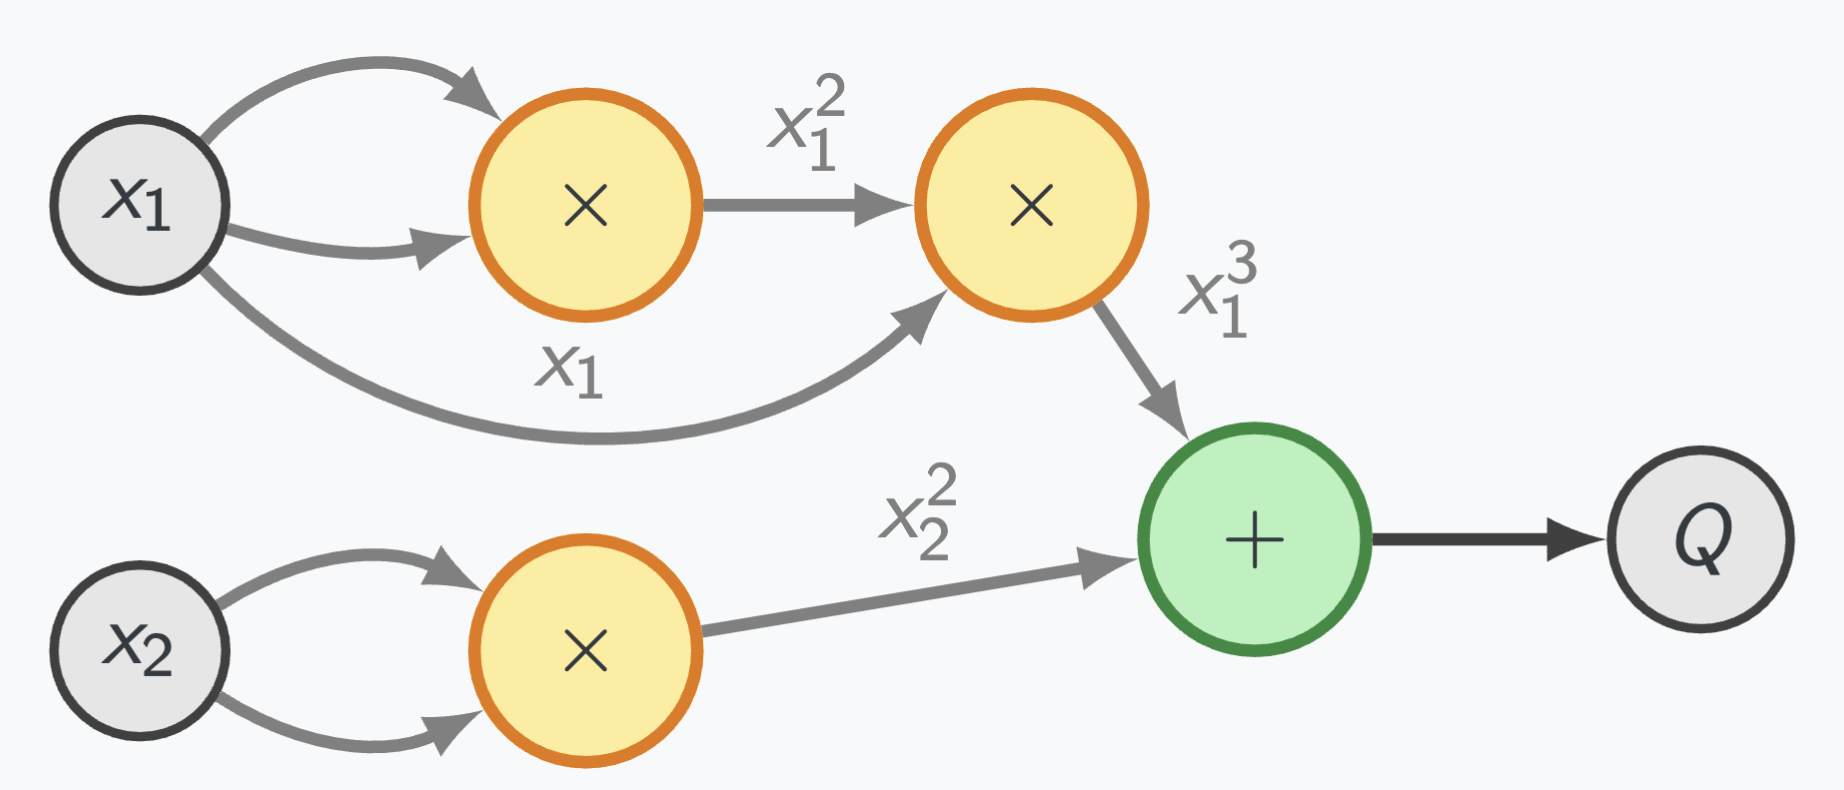
\includegraphics[width=0.8\textwidth]{lectures/images/cover-image-1.png}
    \end{figure}

    \thispagestyle{empty}
    \pagebreak

%  Inverse title page

    \thispagestyle{empty}
    \pagebreak
    
    \pagecolor{white}
    
    \begin{center}
        abstract        
    \end{center}
    
    \thispagestyle{empty}

% --- Table of Contents ---

    \pagecolor{white}

    \tableofcontents

    \pagebreak

% --- Content ---

    \section{Group Theory and Polynomials}

     \subfile{lectures-105-135/1-math}

    \section{Basics of Security Analysis}\label{section:math-crypto-2}

    \subfile{lectures-105-135/2-math-and-crypto}

    \section{Field Extensions and Elliptic Curves}

    \subfile{lectures-105-135/3-ec}\label{section:field_extensions}

    \section{Projective Coordinates and Pairing}

    \subfile{lectures-105-135/4-pairing}

    \section{Commitment Schemes}

    \subfile{lectures-105-135/5-commitments}

    \section{Introduction to Zero-Knowledge Proofs}

    \subfile{lectures-105-135/6-intro-zk}

    \section{Sigma Protocols}

    \subfile{lectures-105-135/7-sigma}

    \section[Introduction to SNARKs]{Introduction to SNARKs. Arithmetic Circuits. R1CS}

    \subfile{lectures-105-135/8-circuits}\label{secation:circuits}

    \section[Quadratic Arithmetic Program]{Quadratic Arithmetic Program. Probabilistically Checkable Proofs}

    \subfile{lectures-105-135/9-qap-pcp}

    \section[Pairing-based SNARKs]{Pairing-based SNARKs. Pinocchio and Groth16}

    \subfile{lectures-105-135/10-groth}

    \section{Circom}

    \subfile{lectures-105-135/11-circom}

    \section{PlonK}

    \subfile{lectures-105-135/12-plonk}

    % Contacy page

    \newpage
    \pagestyle{empty}
    
    \ifodd\value{page}
        \newpage
    \fi
    
    \vspace*{\fill}
    
    \begin{center}
        contact@distributedlab.com
    \end{center}
    
    \vspace*{\fill}

\end{document}
